\chapter{Background}\label{Background}

\section{Automatic Music Transcription}

In general, transcription refers to the process of retrieving information from audible data, such as sounds or music. Specifically when applied on music, the information we seek is often an annotation in music notation. This is what is referred to as \textit{music transcription}. Generally, transcribing a musical piece is expensive, requiring both extensive experience within a specific instrumental field, as well as a lot of manual, time-consuming work. Early on in 1986, Martin Piszczalski stated that \textit{"The learned, human skill of transcribing music is one of the most sophisticated auditory-based pattern-recognition tasks that humans perform."}~\cite{10.5555/15202}. A decade prior he helped introduce the term \acrfull{AMT} covering a field in which now, many years later, has evolved significantly~\cite{piszczalski1977automatic}.

\subsection{Transcription using Deep learning}
Currently, the majority of state-of-the-art within \gls{AMT} utilizes deep learning~\cite{8350302, signals4040042, jamshidi2024machine}. With enough data one can train a \gls{DNN} to, given an input sequence of music, automatically output a transcribed sequence representing musical notation. Musical notation such as this could be extensive in their information, but by far the most important parts could be reduced down to \textit{"which instruments are playing"} and \textit{"when are they playing"}.

Relating this to a common deep learning task, this could be described as a multi-label sequence tagging/sequence labelling task. For each element in an input sequence output a combination of one or more labels. Each element within this sequence represents a timestep in the audio recording, with a combination of labels representing one or more instruments being played. This constitutes the most basic form of \gls{AMT}.

\begin{figure}[H]
    \centering
    \begin{tikzpicture}

\node[
    label=north:{\large{Music}}
] (music) at (-5.5, 0) {
    \begin{tikzpicture}
        \node at (0, 0) {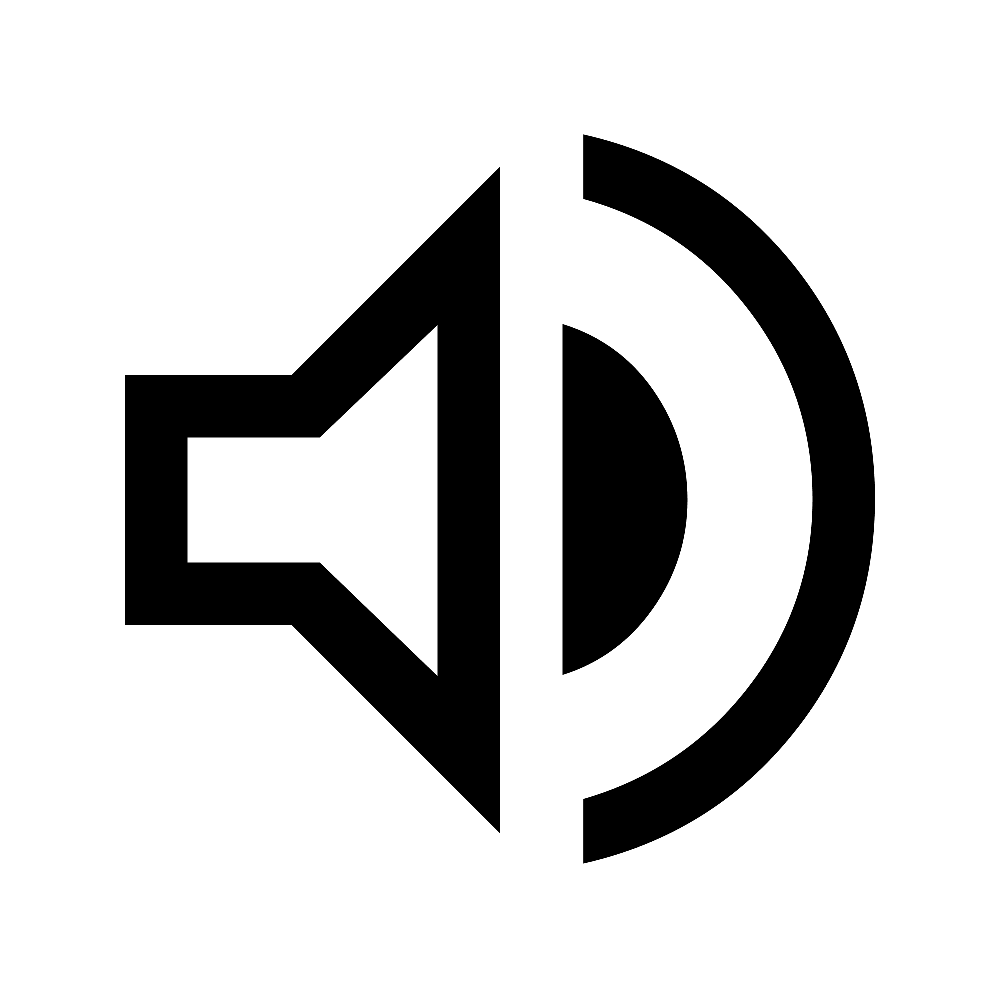
\includegraphics[scale=0.06]{figures/speaker.png}};
        \node [rotate=30, scale=1.6] at (1.1, 0.85) {\AAcht};
        \node [rotate=-30, scale=1.2] at (1, -0.75) {\Acht};
    \end{tikzpicture}
    };

\node[
    label={[label distance=1.08em]north:{\large{Deep Learning}}},
    rectangle,
    draw,
    thick,
    minimum height=5em,
    minimum width=10em,
] (nn) at (0, 0) {\large{Neural Network}};

\node[
    label={[label distance=1.08em]north:{\large{Transcription}}},
    minimum height=5em,
] (transcription) at (5.5, 0) {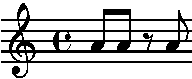
\includegraphics[scale=1.0]{lilypond/amt.cropped.pdf}};

\draw[->, thick] (music.east) -- (nn.west);
\draw[->, thick] (nn.east) -- (transcription.west);

\end{tikzpicture}

    \caption{An abstract visualization of the \acrfull{AMT} process using deep learning. Music is input, processed by a neural network, and ultimately converted into a symbolic transcription.}
    \label{AMTFigure}
\end{figure}

\section{Audio}

Sound is described by \textit{"the sensation caused in the nervous system by vibration of the delicate membranes of the ear."}~\cite{1953fundamentals}. In short, sound is the human perception of acoustic waves in a transition medium, like air. These waves, consisting of vibrating molecules, get sensed by our auditory organs and perceived by the brain. 

Thus sound can be described as the propogation and perception of waves. Mathematically, waves can be studied as signals~\cite{8454362}. To represent these sounds digitally, as \textit{audio}, one can express these waves as a signal, giving rise to the \textit{waveform}. The waveform is a timewise representation of a signal as a graph, charting the amplitude, or strength of the signal, over time.

\begin{figure}[H]
    \centering
    \begin{tikzpicture}

% Waveform signal
\draw[
domain=0:9, 
samples=300,
smooth,
variable=\x,
blue,
ultra thick,
shift={(-4.5, 2.2)},
] plot ({\x},{sin((3.05*\x + 0.3) r) * 0.8});
\node at (0, 3.5) {\large Digital Waveform};
    
% Pressure wave
\node[
    label=south:{\large Acoustic Sound Wave}
] (pressure) at (0, 0) {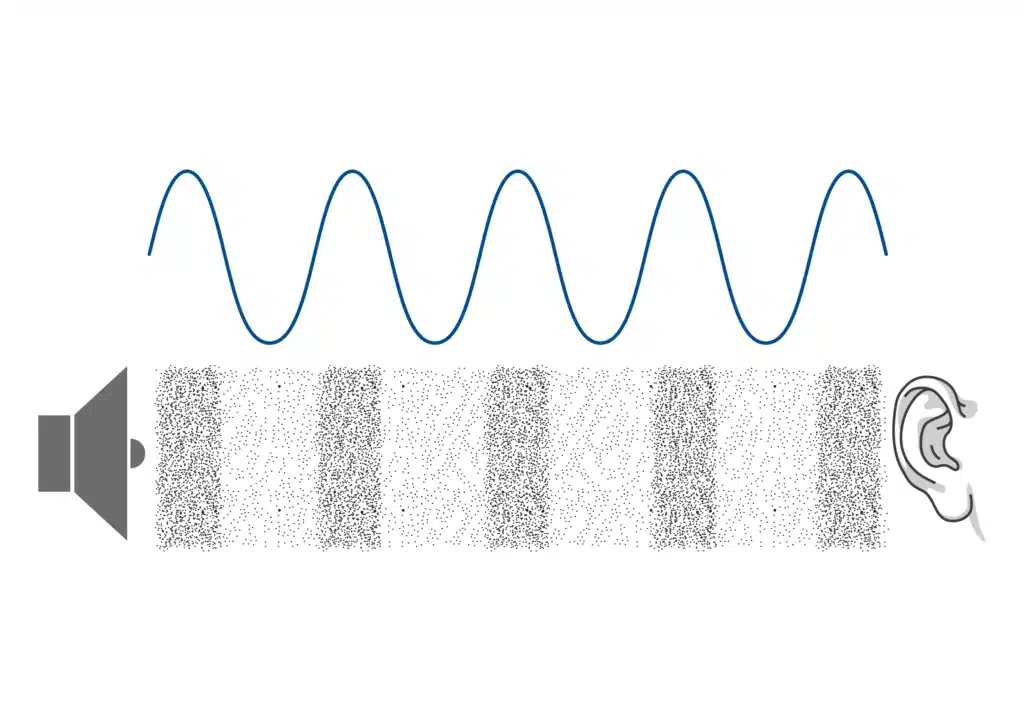
\includegraphics[trim={5.25cm 5.5cm 4.75cm 12.5cm},clip,scale=0.35]{figures/waveform}};

% Speaker
\node[left=-0.25cm of pressure] {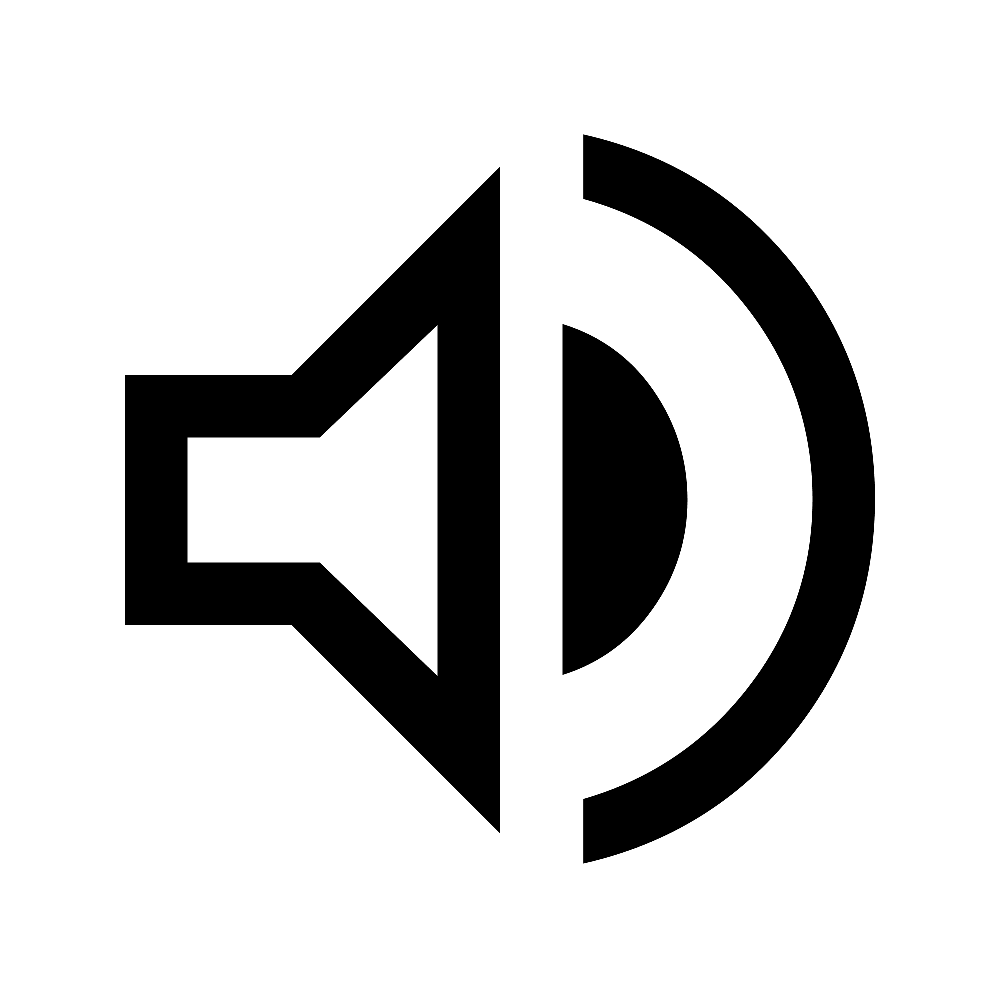
\includegraphics[scale=0.065]{figures/speaker.png}};

% Ear
\node[right=-0.25cm of pressure] {\scalebox{-1}[1]{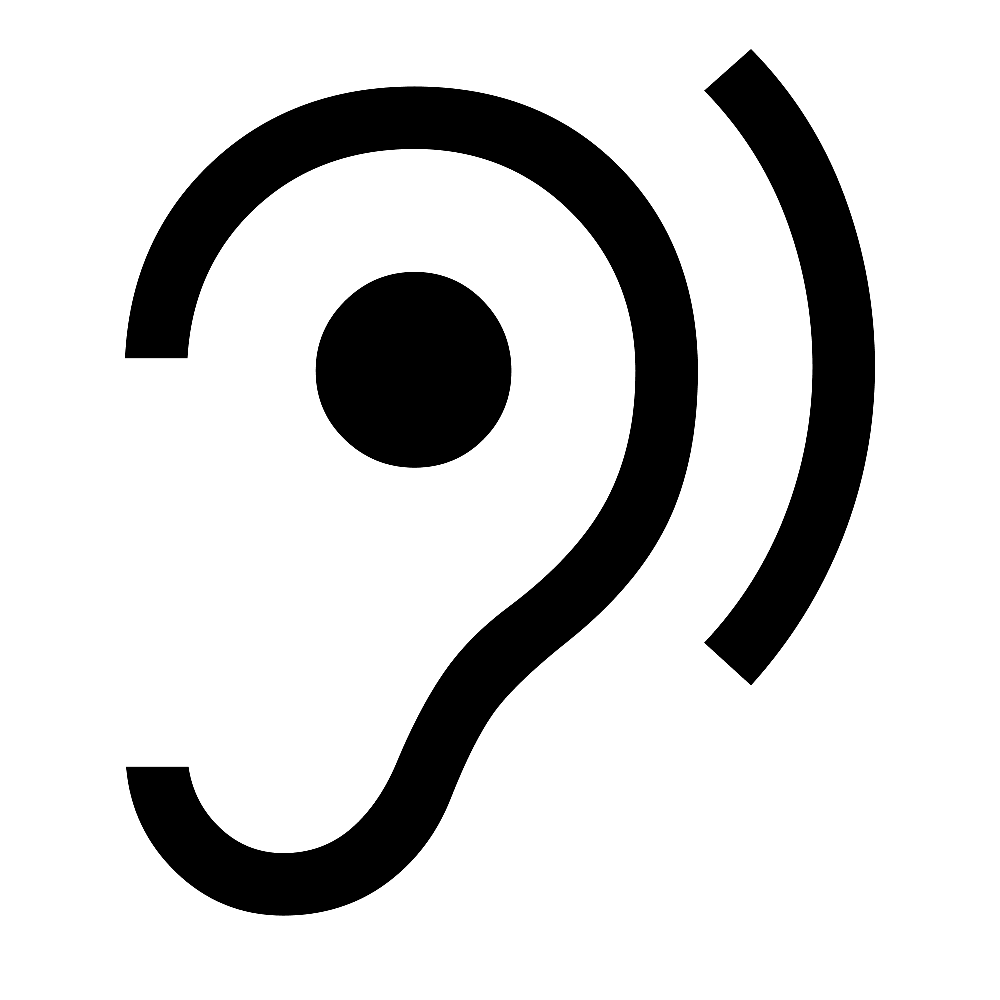
\includegraphics[scale=0.065]{figures/ear.png}}};

\end{tikzpicture}
    \caption{The relationship between an acoustic sound wave and its corresponding digital waveform. The waveform represents variations in the air pressure over time. Regions of higher and lower pressure in the sound wave correspond to \textit{peaks} and \textit{troughs} in the waveform, respectively.}
    \label{WaveformFigure}
\end{figure}

For monophonic sound, this waveform is a one-dimensional representation. Even though this is an excellent way of storing audio digitally, informationally it is very dense. Although there do exist deep learning models working directly with these waveforms, such as Oord et al.'s WaveNet~\cite{oord2016wavenetgenerativemodelraw}, the task of parsing and perceiving such a signal is a complex one. Luckily, there exists some processing techniques which can be applied to a waveform, lowering its complexity whilst keeping information intact.

\subsection{Fourier Transform}

The Fourier Transform is a mathematical transformation which, given a signal and frequency, computes the frequency's significance, or intensity, in the original signal. As we've established, audio is represented as a signal, meaning we therefore can use this transform, turning an audio signal into frequency space. 

The fourier transform is a complex transformation. Specifically given a signal $f$, we can compute the integral \[ \widehat{f}(\xi) = \int^{\infty}_{-\infty}{f(x)e^{-i2\pi \xi x} dx} \] for a frequency $\xi \in \mathbb{R}$, computed over all values $x \in \mathbb{R}$ representing time, resulting in a \textit{complex} number on the form $\widehat{f}(\xi) = a + bi$. This number consists of a \textit{real} part $a$ and an \textit{imaginary} part $b$. We can represent this complex number in polar form \[ a + bi = re^{i\theta}, \] where $r = \sqrt{a^2 + b^2}$ denotes the magnitude (amplitude) and $\theta = \arctan{(\frac{b}{a})}$, adjusted for the right quadrant, computes the phase of the respective frequency in the original signal $f$. Frequencies with higher amplitudes play a more prominent role in shaping the original sequence, indicating a greater significance. This information is what allow us to figure out which frequencies a signal is made out of and how each frequency contributes. 

By doing such a transform we turn our temporal data, like a waveform, into spectral data, its \textit{spectrum}. This inuitively \textit{untangles} our signal into its respective base frequencies. By ridding our data with the highly dense temporal aspect, replacing it with a more informationally independent and sparse spectral representation, a transformation such as this could lessen the complexity of the task, making the audio easier to \textit{understand}; in a metaphorical sense.

\begin{figure}[H]
    \centering
    \hspace*{-1.3cm}
    \begin{tikzpicture}
        \node at (0, 0) {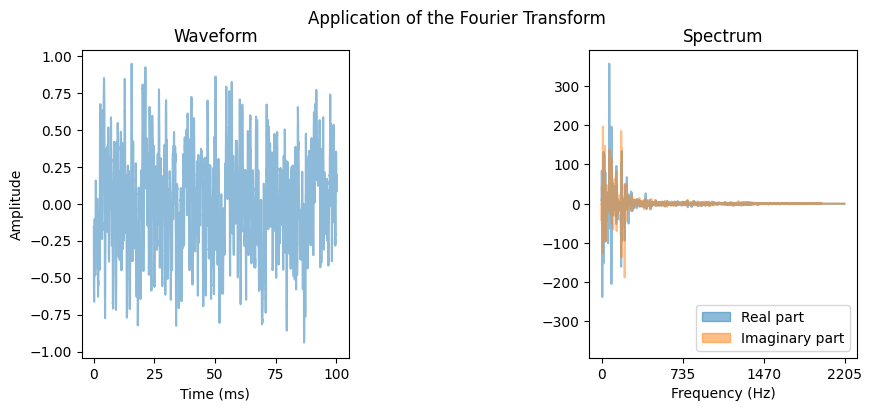
\includegraphics[scale=0.8]{figures/fouriertransform}};
        \draw[->] (-1, 0) -- (1.75, 0) node[above, midway, font=\footnotesize] {Fourier Transform};
    \end{tikzpicture}
    \caption{The Fourier Transform decomposes a waveform into its frequency components. The time-domain waveform signal on the left is measured in amplitude, where higher amplitudes correspond to higher sound wave air pressure levels. The frequency-domain spectrum on the right displays the amplitude of each frequency, indicating its contribution to the original signal.}
    \label{FTFigure}
\end{figure}

Note that the Fourier Transform is invertible, meaning that the original signal can be reconstructed from its frequency components via an inverse transformation. This property is fundamental to the Fourier Transform's integral and widely exploited within signal processing.

\subsection{Discrete Fourier Transform}

The Fourier Transform is defined as an integral over continuous time. On computers, instead of storing signals continuously we instead store signals using a discrete number of samples. Each signal's \textit{sampling rate} describes how many samples a signal contains per second of audio, and is denoted in \textit{Hz}.

To extract frequency values from these signals, we instead have to use the \gls{DFT}. Intuitively this works identically to the normal Fourier Transform, just ported to work on discretely sampled signals. It is given by the formula \[ X_k = \sum^{N - 1}_{n=0}{x_n \cdot e^{-i 2\pi \frac{k}{N} n}}, \] where $k$ denotes a certain frequency bin and $N$ the number of discrete samples. Note that contrary to the normal Fourier transformer, instead of computing the magnitude of each specific real-valued frequency, we instead compute the magnitude of frequencies covered by certain frequency bins. The number, or granularity, of these bins are directly dependent on the number of samples $N$, and the respective frequencies covered by each bin is given by the signal's sampling rate.

\subsection{Nyquist frequency}

When a continuous signal, such as an audio wave traveling through the air, is discritized by recording it on a computer, some information may be lost in the process. The discrete representation of the signal is an \textit{approximation} which quality is directly dependent on the sampling rate. The higher the sampling rate, the \textit{closer} we are to the original, continuous signal. However a higher sampling rate comes at the cost of needing to store these signals at a higher precision. A lower sampling rate would need less information stored, but this could also mean a less precise signal approxmation.

\textit{Aliasing} is the phenomenon where new, incorrect frequencies emerge in undersampled signals. The \textit{Nyquist frequency}, defined as half the sampling rate, represents the highest frequency that can be accurately captured by a discrete signal. Thus to prevent aliasing, the sampling rate must be at least twice the maximum frequency present in the original signal.

\begin{figure}[H]
    \centering
    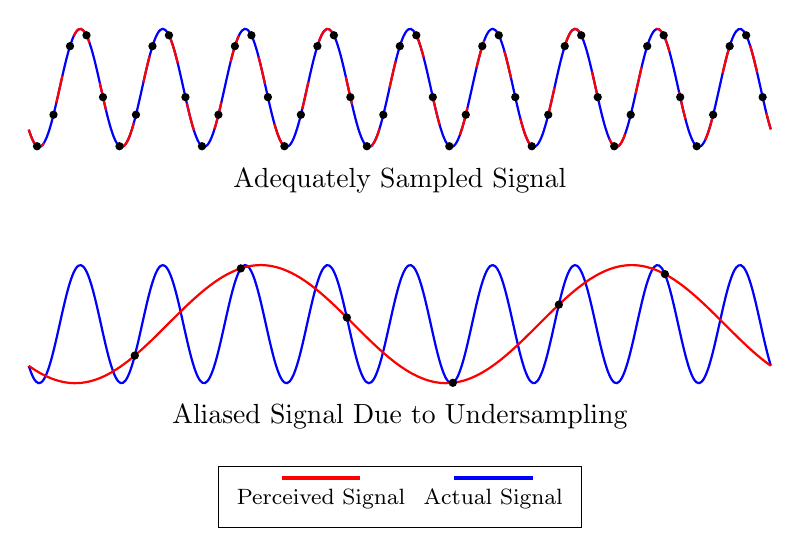
\begin{tikzpicture}[scale=1.5]

% Above Signal
\draw[
domain=0:2*pi, 
samples=300,
smooth,
variable=\x,
blue,
thick,
shift={(0, 2)}
] plot ({\x},{sin((9*\x - 3*pi/4) r)/2});

% Above Perceived
\draw[
domain=0:2*pi, 
samples=300,
smooth,
variable=\x,
red,
thick,
dash pattern={on 10pt off 15pt},
shift={(0, 2)}
] plot ({\x},{sin((9*\x - 3*pi/4) r)/2});

% Scatter Adequate Samples
\foreach \i in {1,...,45} {
    \pgfmathsetmacro\xsamp{2*pi*(\i-0.5)/45}
    \pgfmathsetmacro\ysamp{sin((9*\xsamp - 3*pi/4) r)/2}
    \fill (\xsamp, \ysamp + 2) circle (1pt);
}

% Above Text
\node[
anchor=north, 
] at (pi, 1.4) {Adequately Sampled Signal};


% Below Signal
\draw[
domain=0:2*pi, 
samples=300,
smooth,
variable=\x,
blue,
thick
] plot ({\x},{sin((9*\x - 3*pi/4) r)/2});

% Below Perceived
\draw[
domain=0:2*pi, 
samples=100,
smooth,
variable=\x,
red,
thick
] plot ({\x},{sin((2*\x - 3*pi/4) r)/2});

% Scatter Aliasing Samples
\foreach \i in {1,...,6} {
    \pgfmathsetmacro\xsamp{2*pi*\i/7}
    \pgfmathsetmacro\ysamp{sin((9*\xsamp - 3*pi/4) r)/2}
    \fill (\xsamp, \ysamp) circle (1pt);
}

% Below Text
\node[
anchor=north, 
] at (pi, -0.6) {Aliased Signal Due to Undersampling};


% Legend
\tikzset{
    legend entry/.pic={
        \draw[pic actions, line width=1.5pt] (-0.5, 0) -- (0.5, 0);
    }
}
\matrix [draw, below] at (pi, -1.2) {
    \pic[red]{legend entry}; &  \pic[blue]{legend entry}; \\
    \node[font=\footnotesize] {Perceived Signal}; &  \node[font=\footnotesize] {Actual Signal}; \\
};

\end{tikzpicture}
    \caption{Example of aliasing due to undersampling. The original signal has a true frequency of 9~Hz. In the upper plot, sampling at a sufficiently high rate of 45~Hz allows the signal to be perceived and reconstructed accurately. In the lower plot, however, a lower sampling rate of 7~Hz causes aliasing, and the signal is incorrectly perceived as having a frequency of 2~Hz.}
    \label{AliasingFigure}
\end{figure}

In the case of the \gls{DFT}, it directly follows that the maximum frequency from which accurate information can be extracted is proportional to the signal's sampling rate. Specifically, it is equal to the signal's Nyquist frequency.

\subsection{Fast Fourier Transform}

Keen-eyed computer scientists may note that the \gls{DFT} has a time complexity of $\mathcal{O}(n^2)$, since it requires summing over $N$ values for each of the $N$ different frequencies. As a result, the \gls{DFT} scales poorly in regards to input size. For instance, given that the standard audio sampling rate is $44.1 \text{kHz}$, the computational cost becomes significant, making the \gls{DFT} impractical for real-time or large-scale signal analysis~\cite{pras2010sampling}.

The \gls{FFT} algorithm addresses this limitation by computing the same result as the \gls{DFT}, but with a time complexity of $\mathcal{O}(n\log{n})$ instead. Described by Gilbert Strang as \textit{"the most important numerical algorithm of our lifetime"}~\cite{strang1993wavelet}, the \gls{FFT} effectively solves the prior scaling problem, allowing us to efficiently extract spectral information from a signal even at high sampling rates.

There exist several different implementations of the \gls{FFT}. Among them, the Cooley–Tukey algorithm is by far the most widely used, and optimizes its calculations through a \textit{divide and conquer} approach, reducing redundant computation by reusing intermediate results~\cite{d3ea2d52-5ab2-3128-8b80-efb85267295d}.

\subsection{Short-time Fourier Transform}

The Fourier Transform comes with certain limitations; most notably in how, by transforming a signal into the frequency domain, we lose its temporal structure. Although this loss of time information may be acceptable for certain tasks, it poses a challenge for applications like music transcription and \gls{ADT} where timing of events is vital. So far, we've seen how the Fourier Transform unravels the frequency content of a signal as a whole. But what happens if we had applied it to smaller, localized partitions of the signal instead?

This leads us to the \gls{STFT}. Rather than transforming the entire signal at once, the \gls{STFT} applies the Fourier Transform to smaller, overlapping \textit{windows} of the signal. This allows us to extract frequency information while preserving much of its temporal resolution. The result is a two-dimensional representation, revealing the intensity of different frequencies over time.

\begin{figure}[H]
    \centering
    \begin{tikzpicture}

% Signal
\node[
    %label=north:{\Large{Application of the Short-Time Fourier Transform}},
    label=east:{\Huge{\textbf{\dots}}},
    label={[label distance=0.6cm]west:{\large{Signal}}}
] (signal) at (0, 0) {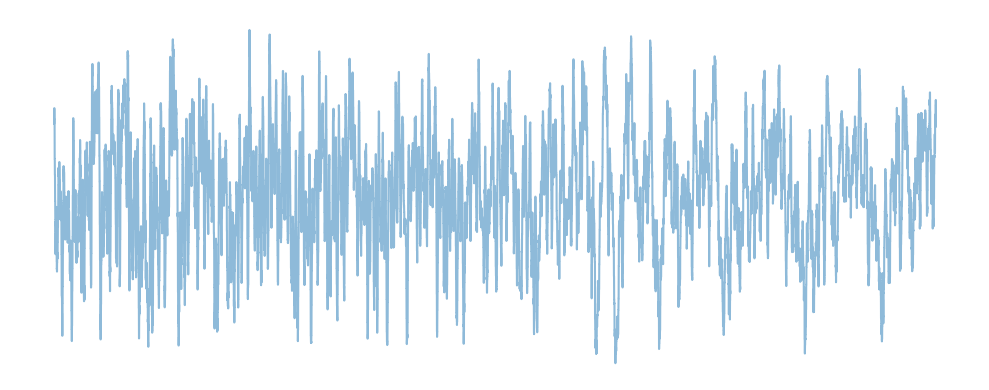
\includegraphics[scale=0.42]{figures/stftfull}};


% Window
\node[
    label=east:{\Huge{\textbf{\dots}}},
    label=west:{\large{Windows}},
    below=0.3cm of signal,
    xshift=-0.2cm
] (windows) {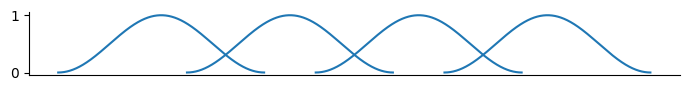
\includegraphics[scale=0.62,trim={0 0.25cm 0 0.2cm},clip]{figures/stftwindows}};

% Window Arrows
\draw[<->] ($(windows.north west) + (1.05, 0)$) -- ($(windows.north) - (1.25, 0)$) 
node[above, midway] (windowlabel) {\footnotesize{Window Length}};
\draw[<->] ($(windows.south west) + (1.05, 0)$) -- ($(windows.south) - (2.5, 0)$) 
node[below, midway] {\footnotesize{Hop Length}};


% Windows
\node[
    below=2cm of windowlabel
] (window0) {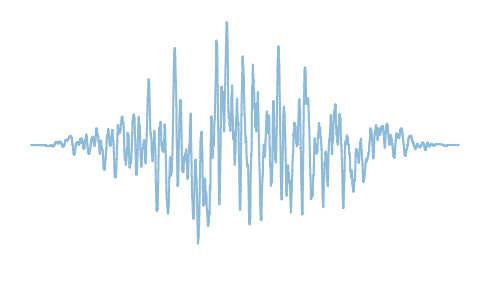
\includegraphics[scale=0.35]{figures/stftwindow0}};
\node[
    below right=-1.75cm and -1.8cm of window0,
    label={[label distance=3cm]west:{\parbox{2.5cm}{\centering \large{Window \\ Partitioning}}}}
] (window1) {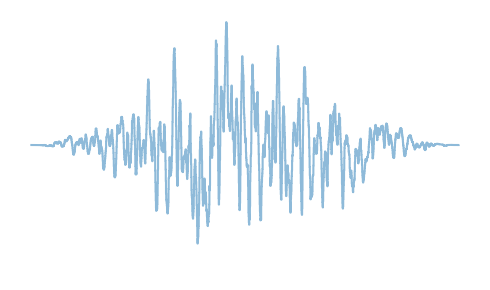
\includegraphics[scale=0.35]{figures/stftwindow1}};
\node[
    below right=-1.75cm and -1.8cm of window1,
    label={[rotate=-45]south east:{\Huge{\textbf{\dots}}}}
] (window2) {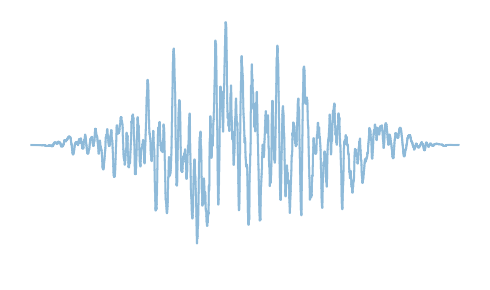
\includegraphics[scale=0.35]{figures/stftwindow2}};


% FFTs
\coordinate (fftarrow) at ($(window1.west |- window2.north) + (0, -1)$);
\draw[->, thick] (fftarrow) -- ($(fftarrow) + (0, -2.45)$) node[left, midway] {\large{FFT}};

\node[
    label=east:{\Huge{\textbf{\dots}}},
    below=1.25cm of window2,
    label={[label distance=-0.25cm]north:{\footnotesize{FFT Output 3}}}
] (fft2) {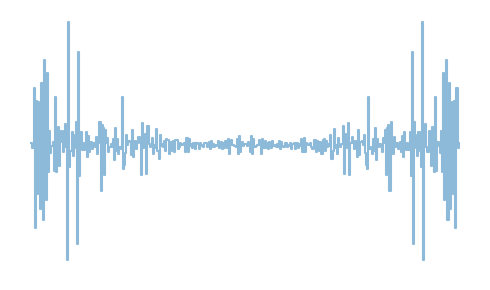
\includegraphics[scale=0.2]{figures/stft2}};
\node[
    left=0.15cm of fft2,
    label={[label distance=-0.25cm]north:{\footnotesize{FFT Output 2}}}
] (fft1) {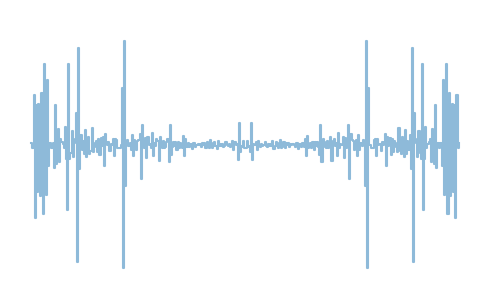
\includegraphics[scale=0.2]{figures/stft1}};
\node[
    left=0.15cm of fft1,
    label={[label distance=-0.25cm]north:{\footnotesize{FFT Output 1}}},
    label={[label distance=0.82cm]west:{\parbox{2.5cm}{\centering \large{Frequency \\ Spectra}}}}
] (fft0) {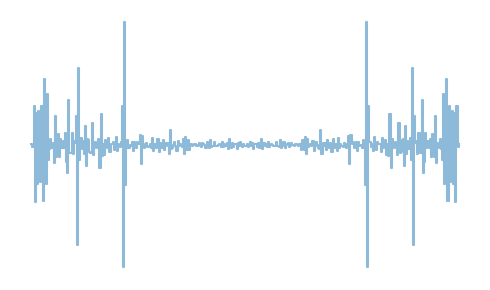
\includegraphics[scale=0.2]{figures/stft0}};

\end{tikzpicture}
    \caption{Application of the \gls{STFT} to a signal. The original waveform is multiplied by multiple offset window functions, producing a set of overlapping signal partitions. The \gls{FFT} is then applied to each partition individually, resulting in a sequence of frequency spectra that preserve localized time–frequency information.}
    \label{STFTFigure}
\end{figure}

The \gls{STFT} has several parameters that affect the structure and resolution of its output; most notably the \textit{window function}, \textit{window length}, and \textit{hop length}. Due to a phenomenon called \textit{spectral leakage}, where spectral information bleeds into other frequencies, a windowing function is applied to each partitioned segment. A common choice is the \textit{Hann window}, illustrated in Figure~\ref{HannWindowFigure}.

The window length plays a crucial role in determining the time–frequency resolution. A longer window improves the frequency resolution, allowing for more precise magnitude estimation of each frequency component, but comes at the cost of reduced time resolution. This is because a large window spans a longer segment of the signal, causing individual windows to overlap more and blur timing information. On the contrary, shorter windows improve temporal precision but blur frequency content, due to each window consequently consisting of fewer samples. This duality is known as the \textit{time–frequency tradeoff}.

The hop length determines how far the window shifts between each segment and directly affects the temporal granularity of the output. A smaller hop length results in more overlap and a finer temporal resolution, but also increases the computational cost by requiring more \glspl{FFT}. Additionally, the hop length defines the time step between frames, allowing each window to be assigned a temporal index.

\begin{figure}[H]
    \centering
    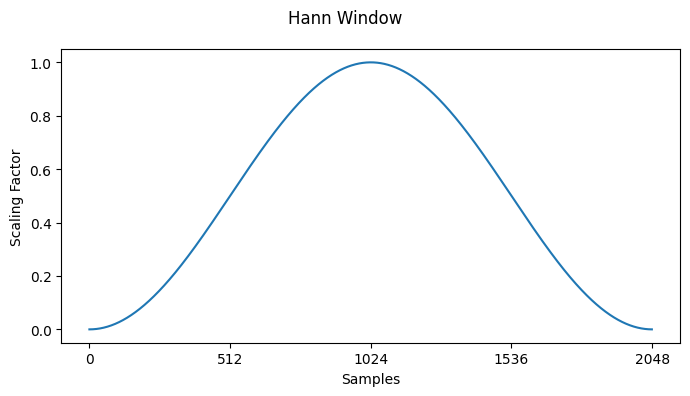
\includegraphics[scale=0.8]{figures/hann}
    \caption{The Hann window function, commonly applied to each partition during the \gls{STFT} to reduce the effects of spectral leakage. It does so by scaling the amplitude of the signal down toward zero at the window's edges. This example shows a window length of 2048 samples.}
    \label{HannWindowFigure}
\end{figure}

For \gls{ADT}, a common configuration is to use the Hann window, with a window size of 2048 samples and a hop length corresponding to 10~ms, i.e., the sampling rate divided by 100~\cite{8350302, vogl2016recurrent,vogl2018multiinstrumentdrumtranscription, signals4040042}.

\subsection{Spectrogram}

The \gls{STFT}, like the standard Fourier Transform, produces complex-valued output. To convert this into strictly real-valued data without discarding meaningful information, we compute the \textit{spectrogram}. Specifically, a magnitude spectrogram is obtained by taking the absolute value of each complex result from the \gls{STFT}.

The result is a two-dimensional, real-valued representation of the signal, where one axis corresponds to time and the other to frequency. While this representation can be modeled as a time series, it is also structurally equivalent to an image. As such, spectrograms are often visualized as heatmaps, offering an intuitive way to observe how frequency information evolves over time.

\begin{figure}[H]
    \centering
    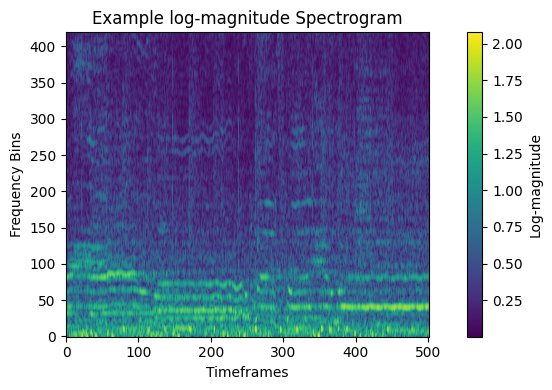
\includegraphics[scale=1.1]{figures/logspectrogram}
    \caption{Log-magnitude spectrogram of the SADTP track \textit{"Red Swan"}, showing the segment from 3:35 to 3:40 minutes. The spectrogram is computed using 2048 \glspl{FFT}, with a window length of 512 samples and a hop length corresponding to 10~ms. Only the first 420 frequency bins are visualized. The color represents the log-magnitude of each time–frequency bin.}
    \label{SpectrogramFigure}
\end{figure}

The number of frequency bins (represented on the y-axis of Figure \ref{SpectrogramFigure}) in a spectrogram is equal to half the number of \glspl{FFT} used in its computation. These bins contain information about linearly spaced frequencies, ranging from 0~Hz up to the Nyquist frequency of the signal. The number of time frames (the x-axis) is determined by the hop length of the \gls{STFT}, with smaller hop lengths resulting in a greater number of frames. In this way, one has significant control over the dimensionality of the spectrogram through parameter selection. 

One drawback of the spectrogram is that it discards all information about signal's phase. As previously mentioned, phase is encoded in the angle of each complex value, which is lost when computing the magnitude. This means it is not possible to perfectly reconstruct the original signal from a magnitude-only spectrogram. However, approximate reconstruction is possible using iterative algorithms such as Griffin–Lim~\cite{1164317}.

\subsection{Loudness of Magnitude}

The human perception of loudness is approximately logarithmic. A soundwave that carries ten times more energy is not perceived as ten times louder. Instead, a doubling in perceived loudness corresponds roughly to a 10~\gls{dB} increase in signal amplitude. The \acrlong{dB} is a relative unit of measurement that expresses the power the ratio between two signals, where an increase of 1~\gls{dB} corresponds to a power ratio of $10^\frac{1}{10}$. The power of a signal is computed as the square of its magnitude. 

This relationship has two major consequences. First, the magnitude scale used in standard spectrograms does not align with human perception of loudness; quiet and loud signals may differ significantly in magnitude, even if they perceptually seem close. Second, this mismatch causes the standard (linear) spectrogram to be highly variable in its magnitude representation, often making it difficult to identify quieter frequency components among louder ones.

To address this, a log-magnitude spectrogram is often used (as in Figure \ref{SpectrogramFigure}), which applies a logarithmic transformation to the magnitudes. This logarithm is typically base 10, aligning with the \acrlong{dB} scale and better reflecting human auditory perception.

\begin{figure}[H]
    \centering
    \hspace*{-1.0cm}
    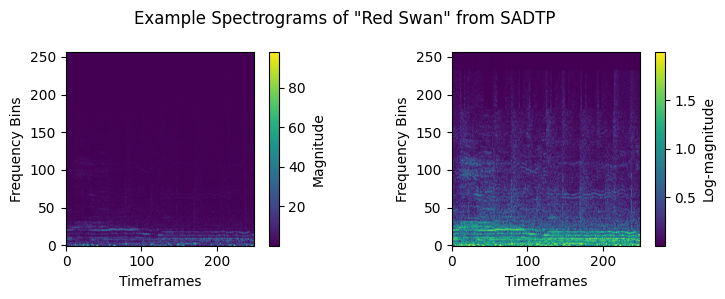
\includegraphics[scale=1.0]{figures/spectrogramlogspectrogram}
    \caption{Comparison between a linear magnitude spectrogram and a log-magnitude spectrogram. When scaled linearly, differences in magnitude are harder to distinguish, especially for quieter frequency components. The logarithmic scale makes both loud and quiet components visually more distinguishable.}
    \label{SpectrogramLogspectrogramFigure}
\end{figure}

\subsection{Filters}

Signal frequencies and human perception have a non-linear relationship. Just as loudness is perceived on a logarithmic scale, so too is pitch. Humans perceive logarithmic differences in frequency as a linear difference in pitch, and are more sensitive to changes in lower frequencies than in higher ones. For example, the notes $\text{A}_2$ and $\text{B}_2$ differ by approximately 13.47~Hz, while $\text{D}_7$ and $\text{E}_7$ differ by nearly 287.70~Hz, yet both are perceived as being one semitone apart, meaning they audibly have the same perceived difference in pitch. Because the frequency bins in a standard spectrogram are spaced evenly in frequency, they do not reflect how pitch is actually perceived, with finer sensitivity in lower regions and coarser sensitivity in higher ones.

To better reflect this, we apply a set of \textit{filters}, each emphasizing a certain frequency range. A filter is typically a triangular weighting function centered at a specific frequency, gradually tapering off toward neighbouring bins. Multiple filters are combined into a \textit{filterbank}, which can be applied to a spectrogram using matrix multiplication. This transforms the frequency axis into a new scale that better aligns with how we hear changes in pitch.

\subsubsection{Mel Spectrograms}

The Mel scale, introduced by Stevens, Volkmann, and Newmann in 1937, transforms the frequency axis into a perceptual pitch scale where equal steps correspond to equal perceived pitch differences. In other words, a linear difference in mels is perceived as a linear difference in pitch. Applying a set of triangular Mel-filters results in a \textit{Mel spectrogram}, a representation widely used in audio-related machine learning tasks. Mel spectrograms have shown successful application in \gls{AMT}.~\cite{gardner2022mt3multitaskmultitrackmusic, chang2024yourmt3+, gong2021astaudiospectrogramtransformer, wolfmonheim2024spectralrhythmfeaturesaudio, 8350302}

\subsubsection{Logarithmic Filters}

While the Mel scale was designed to reflect how humans perceive pitch, a different trend has emerged within \acrfull{ADT}. Rather than using perceptual spacing, many recent \gls{ADT} approaches apply \textit{logarithmically spaced filters}, centered on the note $\text{A}_4$ (440~Hz), resulting in what is referred to in this thesis as a \textit{logarithmically filtered spectrogram}. 

This approach does not attempt to mimic human perception directly, but instead reshapes the frequency axis to reflect musical structure, spacing filters uniformly on a logarithmic scale, with 12 filters per octave to match the 12 semitones in Western music. The filters are designed to cover the human hearing range, from 20~Hz to 20,000~Hz, resulting in a filterbank with 84 frequency bins. Each filter is triangular and area-normalized, such that the area under each filter curve equals 1.

This representation has been adopted in several recent \gls{ADT} studies, particularly by Vogl et al., and is often preferred when preserving musical relationships is important. Compared to Mel spectrograms, it provides a harmonically consistent frequency resolution across octaves, while also reducing input dimensionality~\cite{Vogl2017DrumTV, vogl2018multiinstrumentdrumtranscription, jia2019deep, signals4040042, zehren2024analyzingreducingsynthetictorealtransfer}.

\begin{figure}[H]
    \centering
    \hspace*{-0.6cm}
    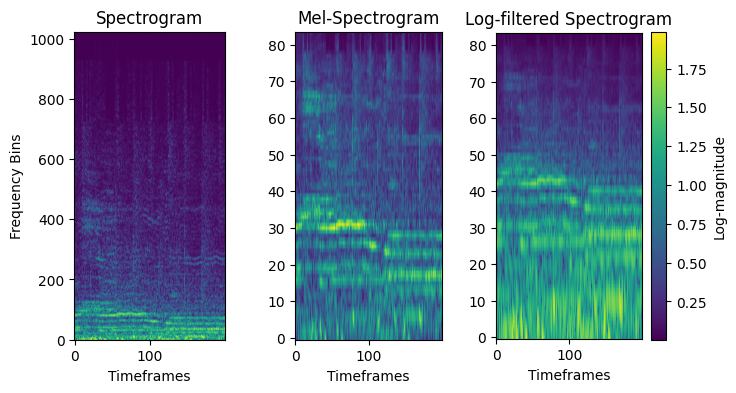
\includegraphics[scale=0.9]{figures/allspectrograms}
    \caption{Comparison between a full spectrogram, a Mel spectrogram, and a log-filtered spectrogram. All are presented on a log-magnitude scale. Both the Mel and log-filtered spectrograms apply 84 area-normalized filters, resulting in a non-linear frequency axis. While the Mel spectrogram emphasizes perceptual resolution, with greater detail in lower frequencies, the log-filtered spectrogram maintains uniform resolution across octaves, aligning with musical intervals.}
    \label{AllSpectrogramFigure}
\end{figure}


\section{Transcription}

Transcription refers to the process of converting an auditory signal, such as music, into a structured representation in another medium. In a musical context, this representation serves as a description of the original performance and may take several different forms.

\subsection{Music Notation}

Modern staff notation is a symbolic transcription systen that provides a structured set of instructions for a musician to reproduce a performance. It has become the standard way of documenting music and is widely used by musicians across many different genres and instruments.

Sheet music written in this notation is typically highly descriptive, containing information such as note onsets, pitch (for pitched instruments), instrument type, velocity, and tempo. Time is represented horizontally from left to right, while pitch or instrument assignment is encoded vertically. For pitched instruments, the vertical position of the note corresponds to its pitch, while for instruments like percussion, the vertical position indicates the specific drum instruments. The duration of the note is denoted through the shape of the notehead, stem, or additional note decorations.

\begin{figure}[H]
    \centering
    \begin{tikzpicture}

\node[anchor=west] at (0, 0) {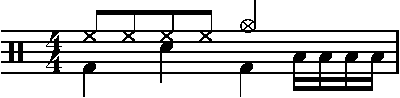
\includegraphics[scale=1.9]{lilypond/drumsheet.cropped.pdf}};

\matrix[
anchor=east,
row sep=-0.205cm
] at (0, 0.1){
    \node[font=\normalsize] {\acrshort{CC+RC}}; \\
    \node[font=\normalsize] {\acrshort{HH}}; \\
    \node[font=\normalsize] {\acrshort{SD}}; \\
    \node[font=\normalsize] {\acrshort{TT}}; \\
    \node[font=\normalsize] {\acrshort{KD}}; \\
};

\end{tikzpicture}
    \caption{An example drum sheet containing all instruments used in a 5-instrument \gls{ADT} task. The instrument associated with each row is shown on the left. From bottom to top, they are the \acrfull{KD}, \acrfull{TT}, \acrfull{SD}, \acrfull{HH}, and \acrfull{CC+RC}.}
    \label{DrumsheetFigure}
\end{figure}

Note that rest marks such as $\HaPa$, $\ViPa$, $\AcPa$, and $\SePa$ may appear in notation transcriptions. These indicate brief silences or pauses in the music. Although they may appear inline with other onset events, they do not represent instrument activity and should not be interpreted as onsets.

\subsection{MIDI Annotations}

\gls{MIDI} is the industry standard for representing and controlling digital music. It is an event-based protocol, encoding sequences of commands used to synthesize or trigger musical sounds. As it is stored in a binary format, \gls{MIDI} is not directly readable to humans without translating it into a more interpretable representation. 

When computers play \gls{MIDI} sequences, the events are parsed in order at a fixed rate, using \textit{note on}/\textit{note off} messages seperated by time deltas. Similar to sheet music, \gls{MIDI} is highly descriptive, capturing information such as pitch, velocity and timing. Intuitively, one might think of \gls{MIDI} as serving the same role for computers as sheet music does for musicians.

Recently, several works in \gls{AMT} have explored generating transcriptions in a \gls{MIDI}-like format, with promising results. Using an \acrshort{NLP} approach, Gardner et al. introduced MT3~\cite{gardner2022mt3multitaskmultitrackmusic}, a model that takes log-Mel spectrograms as input and autoregressively predicts \gls{MIDI} events. This format was further developed by Chang et al. in YourMT3+~\cite{chang2024yourmt3+}, utilizing an \acrshort{LLM} instead.

\begin{figure}[H]
    \centering
    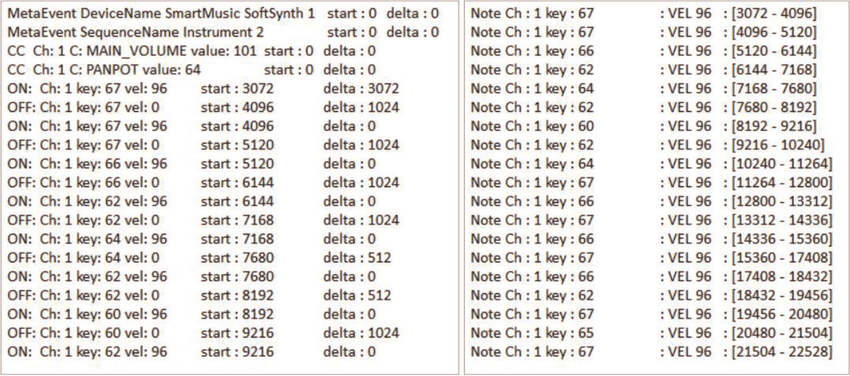
\includegraphics[scale=0.65, trim={0 0 13.8cm 0},clip]{figures/midi}
    \caption{Example MIDI arrangement in text format. The first lines contain metadata, followed by note on/off events. Each event includes temporal information (start, delta), as well as musical attributes such as channel, key, and velocity, which determine the instrument and sound ~\cite{starostenko2019}.}
    \label{MIDIFigure}
\end{figure}

\subsection{Activation Functions}

In machine learning, the task of detecting instrument onsets can be framed as a multi-label sequence labeling problem. For each time frame in a sequence, the model predicts a confidence value (which can be interpreted as a probability), that a given instrument onset occurs at that moment. In the context of \gls{MIR} and \gls{AMT}, it has become common practice to describe these confidence distributions over time as \textit{activation functions} (not to be confused with the activation functions used within neural networks, such as \acrshort{ReLU} or sigmoid)~\cite{schluter2014improved, bock2016joint, Southall2016AutomaticDT, 8350302, vogl2018multiinstrumentdrumtranscription}.

Frame-level prediction of activation functions is a common approach in onset detection for \gls{ADT}, and is the format adopted in this thesis. Each drum instrument's activation function forms a row in a matrix, with time progressing along the columns.

\begin{figure}[H]
    \centering
    \hspace*{-0.5cm}
    \begin{tikzpicture}

% Drum Sheet
\node[
    anchor=east,
    label=north:{\large{Drum Notation}}
] at (0, 0) {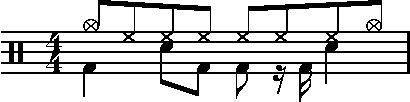
\includegraphics[scale=1.2]{lilypond/activations.cropped.pdf}};


% Activation Functions
\node[
    anchor=south
] at (5, 3.1) {\large{Activation Functions}};

% Cymbals and Ride
\draw[->,
thick
] (0, 0.5) -- (2, 2.5) node[midway, fill=white] {\acrshort{CC+RC}};
\draw[
    anchor=west,
    shift={(2.45, 2.1)}
] (-0.25, -0.1) -- (5.25, -0.1) -- (5.25, 0.9) -- (-0.25, 0.9) -- cycle;
\draw[
    anchor=west,
    color=blue,
    shift={(2.45, 2.1)}
] (-0.25, 0) -- (-0.05, 0) -- (0, 0.8) -- (0.05, 0) -- (4.95, 0) -- (5, 0.8) -- (5.05, 0) -- (5.25, 0);
\foreach \point in {(0, 0.8), (5, 0.8)} {
    \draw[
        color=red,
        shift={(2.45, 2.1)}
    ] \point circle (1.7pt);
}


% Hi-Hat
\draw[->,
thick
] (0, 0.25) -- (2, 1.25) node[midway, fill=white] {\acrshort{HH}};
\draw[
    line width=0.6pt,
    anchor=west,
    shift={(2.45, 0.85)}
] (-0.25, -0.1) -- (5.25, -0.1) -- (5.25, 0.9) -- (-0.25, 0.9) -- cycle;
\draw[
    anchor=west,
    color=blue,
    shift={(2.45, 0.85)}
] (-0.25, 0) -- (0.66, 0) -- (0.71, 0.8) -- (0.76, 0) -- (1.37, 0) -- (1.42, 0.8) -- (1.47, 0) -- (2.09, 0) -- (2.14, 0.8) -- (2.19, 0) -- (2.8, 0) -- (2.85, 0.8) -- (2.9, 0) -- (3.52, 0) -- (3.57, 0.8) -- (3.62, 0) -- (4.23, 0) -- (4.28, 0.8) -- (4.33, 0) -- (5.25, 0);
\foreach \point in {(0.71, 0.8), (1.42, 0.8), (2.14, 0.8), (2.85, 0.8), (3.57, 0.8), (4.28, 0.8)} {
    \draw[
        color=red,
        shift={(2.45, 0.85)}
    ] \point circle (1.7pt);
}


% Snare Drum
\draw[->,
thick
] (0, 0) -- (2, 0) node[midway, fill=white] {\acrshort{SD}};
\draw[
    anchor=west,
    shift={(2.45, -0.4)}
] (-0.25, -0.1) -- (5.25, -0.1) -- (5.25, 0.9) -- (-0.25, 0.9) -- cycle;
\draw[
    anchor=west,
    color=blue,
    shift={(2.45, -0.4)}
] (-0.25, 0) -- (1.37, 0) -- (1.42, 0.8) -- (1.47, 0) -- (4.23, 0) -- (4.28, 0.8) -- (4.33, 0) -- (5.25, 0);
\foreach \point in {(1.42, 0.8), (4.28, 0.8)} {
    \draw[
        color=red,
        shift={(2.45, -0.4)}
    ] \point circle (1.7pt);
}


% Tom-Toms
\draw[->,
thick
] (0, -0.25) -- (2, -1.25) node[midway, fill=white] {\acrshort{TT}};
\draw[
    anchor=west,
    shift={(2.45, -1.65)}
] (-0.25, -0.1) -- (5.25, -0.1) -- (5.25, 0.9) -- (-0.25, 0.9) -- cycle;
\draw[
    anchor=west,
    color=blue,
    shift={(2.45, -1.65)}
] (-0.25, 0) -- (5.25, 0);
\foreach \point in {} {
    \draw[
        color=red,
        shift={(2.45, -1.65)}
    ] \point circle (2pt);
}

% Kick Drum
\draw[->,
thick
] (0, -0.5) -- (2, -2.5) node[midway, fill=white] {\acrshort{KD}};
\draw[
    anchor=west,
    shift={(2.45, -2.9)}
] (-0.25, -0.1) -- (5.25, -0.1) -- (5.25, 0.9) -- (-0.25, 0.9) -- cycle;
\draw[
    anchor=west,
    color=blue,
    shift={(2.45, -2.9)}
] (-0.25, 0) -- (-0.05, 0) -- (0, 0.8) -- (0.05, 0) -- (2.09, 0) -- (2.14, 0.8) -- (2.19, 0) -- (2.8, 0) -- (2.85, 0.8) -- (2.9, 0) -- (3.87, 0) -- (3.92, 0.8) -- (3.97, 0) -- (5.25, 0);
\foreach \point in {(0, 0.8), (2.14, 0.8), (2.85, 0.8), (3.92, 0.8)} {
    \draw[
        color=red,
        shift={(2.45, -2.9)}
    ] \point circle (1.7pt);
}

\end{tikzpicture}
    \caption{Activation function representation for a 5-instrument \gls{ADT} task, corresponding to a drum pattern written in standard staff notation. Each activation function is zero throughout, except at onset positions, where it takes a value of one. The $\SePa$ symbol indicates a sixteenth-note rest in the \gls{KD} instrument, and should not be interpreted as an onset.}
    \label{ActivationsFigure}
\end{figure}

\subsubsection{Peak-picking}

When predicting activation functions, a separate post-processing step is required to convert the continuous confidence distributions into discrete onset events. This is commonly achieved using a standard \textit{peak-picking} algorithm, which isolates and enhances peaks in the activation functions.

The peak-picking algorithm, introduced in its current form by Böck et al.~\cite{Bck2012EvaluatingTO}, defines an onset at time frame $n$ if the predicted activation $\hat{y}_n$ satisfies the following three conditions:
\begin{align*} 
    \hat{y}_n &= \max(\hat{y}_{n - m}, \dots \hat{y}_n, \dots \hat{y}_{n + m}), \\ 
    \hat{y}_n &\ge \text{mean}(\hat{y}_{n - a}, \dots \hat{y}_n, \dots \hat{y}_{n + a}) + \delta, \\
    n &\ge n_\text{last onset} + w.
\end{align*}
Here, $m$ defines the local window size for detecting peaks, $a$ controls how much context is used when averaging surrounding values, $\delta$ sets how far above the average the peak must be, and $w$ defines the minimum spacing between two detected onsets. For appropriately trained deep learning models, Vogl et al.~\cite{vogl2018multiinstrumentdrumtranscription} found that the peak-picking parameters that gave the best results were $m = a = w = 2$ and $\delta = 0.1$. Consequently, these parameter values are also adopted in this thesis.


\section{Automatic Drum Transcription}

As mentioned, \acrfull{ADT} refers to the task of transcribing symbolic drum notation from audio recordings. More specifically, the field can be divided into several subtasks, ordered from simpler to more complex settings~\cite{8350302}. These include:
\begin{itemize}
    \item \acrshort{DSC}: Drum sound classification, which involves identifying the instrument class of isolated, single-event drum recordings.
    \item \acrshort{DTD}: Drum transcription from recordings containing only drum instruments.
    \item \acrshort{DTP}: Drum transcription with percussive accompaniment, where the model must transcribe the drum instruments while ignoring non-drum percussion.
    \item \acrshort{DTM}: Drum transcription from full musical mixtures, where both melodic and percussive instruments are present and only drum onsets should be transcribed.
\end{itemize}

This thesis focuses on the most complex of these tasks, namely \acrfull{DTM}. Intuitively, the goal is to develop a deep learning model that, given input audio in the form of music containing both drums and melodic instruments, can detect and classify drum instrument onsets while selectively ignoring unrelated melodic content. This setting introduces challenges not present in the simpler variants. As Zehren et al.~\cite{signals4040042} note, \textit{"melodic and percussive instruments can overlap and mask eachother..., or have similar sounds, thus creating confusion between instruments"}.

Deep learning has proven to be an effective approach for \gls{DTM}, and a range of architectures have been explored with promising results. Vogl et al.~\cite{Vogl2017DrumTV, vogl2018multiinstrumentdrumtranscription} achieved strong results using both convolutional and convolutional-recurrent networks. Zehren et al.~\cite{signals4040042, zehren2024analyzingreducingsynthetictorealtransfer} emphasized the importance of dataset size and quality, showing that both are critical to achieving strong performance. Most recently, Chang et al.~\cite{chang2024yourmt3+} proposed an autoregressive language-model approach for multi-instrument transcription (\gls{AMT}), with competitive results on \gls{DTM}.

These works highlight that multiple modeling directions remain viable and that further improvements in \gls{ADT} and \gls{DTM} performance are still possible.

\subsection{The Drum Set}

A drum set is a collection of percussive instruments, typically including drums, cymbals, and possibly different auxiliary percussion. While the exact configuration can vary, a standard drum kit typically includes a \gls{SD}, a \gls{KD}, one or more \glspl{TT} (toms), one or more cymbals (\gls{CC} and \gls{RC}), and a \gls{HH} cymbal~\cite{TheDrumHandbook2003}.

\begin{figure}[H]
    \centering
    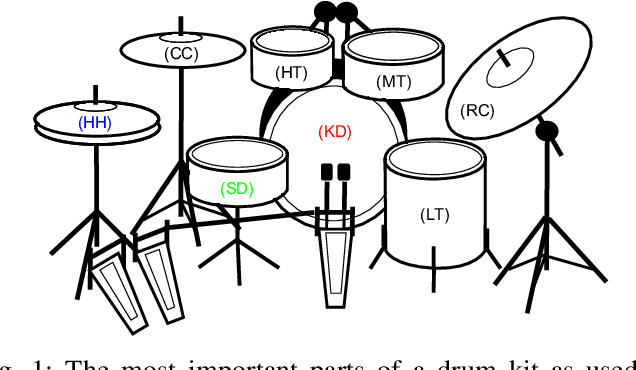
\includegraphics[scale=0.7, trim={0 1cm 0 0},clip]{figures/drumset}
    \caption{The standard drum set configuration, including the \acrfull{KD}, \acrfull{SD}, \acrfull{HH}, \acrfull{CC}, \acrfull{RC}, \acrfull{HT}, \acrfull{MT}, \acrfull{LT}~\cite{8350302}.}
    \label{DrumsetFigure}
\end{figure}

Percussion instruments like those in a drum set stand apart from melodic instruments in that different components, such as the snare, kick, and hi-hat, produce distinctly different acoustic signatures. Even within a single drum, variations in playing technique can significantly affect the resulting sound or \textit{"audible footprint"}. The snare drum, kick drum, and hi-hat differ significantly in timbre, frequency range, loudness, and function, making them acoustically and musically distinct.

\begin{figure}[H]
    \centering
    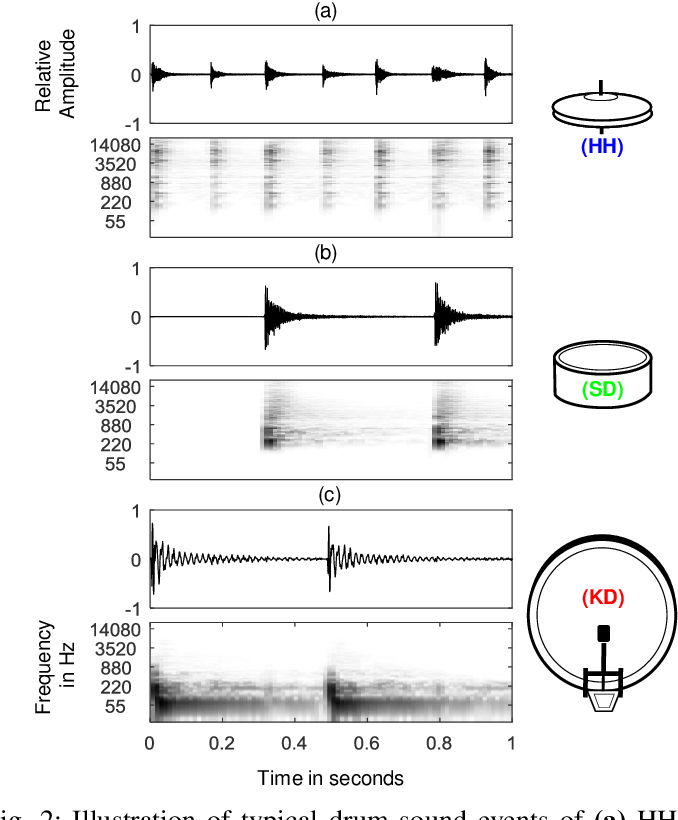
\includegraphics[scale=0.6, trim={0 1cm 0 0},clip]{figures/drumsettimbre}
    \caption{Examples of the different audible footprints of drum set components. Plotted are the waveforms of three drum instruments played at varying patterns, each paired with a corresponding spectrogram. The panels highlight how each instrument's events produce distinct patterns in both the time and frequency domains~\cite{8350302}.}
    \label{DrumsetTimbreFigure}
\end{figure}

\subsection{Transcription Task}

Understanding the transcription pipeline, specifically in the context of \gls{ADT}, is essential for this thesis. The process begins with a raw audio waveform representing the musical recording to be transcribed, typically segmented into smaller, non-overlapping partitions~\cite{vogl2018multiinstrumentdrumtranscription, gardner2022mt3multitaskmultitrackmusic}. Each segment is transformed into a spectrogram, which captures the frequency content over time while reducing temporal resolution, making it easier for models to interpret. 

The spectrogram is then passed into an \gls{ADT} model, such as a \gls{DNN}, which predicts, for each time frame, the likelihood that a given drum instrument is played. These continuous probability estimates, commonly referred to as activation functions, are then post-processed into a more interpretable format, such as discrete onsets or drum notation.

\begin{figure}[H]
    \centering
    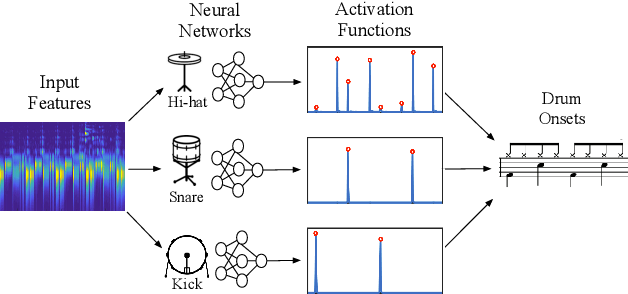
\includegraphics[scale=0.7]{figures/adtpipeline.png}
    \caption{Example of a typical \gls{ADT} pipeline. Given an input spectrogram, the model predicts activation functions for each instrument, which are then quantized into drum onsets and converted into symbolic sheet music~\cite{Southall2016AutomaticDT}.}
    \label{ADTFigure}
\end{figure}

Designing such a pipeline involves several key choices. For instance: How are the input and output of a model structured? While the input here is always a spectrogram, its size and structure can vary depending on parameters such as window length, hop length, and number of frequency bins, as discussed previously. The model's output is also structured as a sequence, with length tied to the input's time resolution and dimensionality determined by the number of instruments being transcribed.

Early work in \gls{ADT} often adopted a 3-instrument setup, predicting only the \acrfull{KD}, \acrfull{SD} and \acrfull{HH}~\cite{vogl2016recurrent}. While this configuration offered a useful proof-of-concept for early model development, it omits essential components of the drum set. To better capture realistic use cases, I instead use a 5-instrument setup, which also includes cymbals (combining both \acrfull{CC} and \acrfull{RC}) and \acrfull{TT} (covering all toms). This adds complexity to the problem but allows the system to represent the full standard drum kit.


\section{Performance Measure}

\subsection{Correct Predictions}

\gls{ADT} models predict instrument onsets on a frame-level basis. To account for slight misalignments between predicted and ground truth events, evaluation is typically performed using a \textit{tolerance window}, where a prediction is considered correct if it falls within a fixed time window around the reference onset, commonly between 25~ms and 50~ms~\cite{vogl2016recurrent}. This approach shifts the evaluation focus from framewise labels to discrete event matching and introduces challenges when defining standard classification metrics.

\subsection{Accuracy}

Although accuracy is a widely used performance measure in classification, it is ill-suited for \gls{ADT}. Most frames contain no onsets, creating a heavy class imbalance that allows a naïve model to achieve high accuracy by simply predicting silence. Moreover, due to the event-based evaluation and tolerance window, the number of \glspl{TN} are generally undefined, rendering the standard accuracy formula:\[ \text{Accuracy} = \frac{\text{TP} + \text{TN}}{\text{TP} + \text{TN} + \text{FP} + \text{FN}},\] inapplicable in practice.

\subsection{F1-score}

Due to the issues outlined above, the \textit{F1-score} has become the standard evaluation metric in \gls{ADT}. It balances two competing objectives: \textit{precision}, which measures the proportion of correct predictions among all predicted events; \[ \text{Precision} = \frac{\text{TP}}{\text{TP} + \text{FP}},\] and \textit{recall}, which measures the proportion of correctly predicted events among all actual events; \[ \text{Recall} = \frac{\text{TP}}{\text{TP} + \text{FN}}. \]

High precision indicates that the model rarely produces \glspl{FP} (i.e., it predicts an onset only when there truly is one), while high recall indicates that the model rarely produces \glspl{FN} (i.e., it doesn't predict an onset only if there truly isn't one). The F1-score captures both by computing their harmonic mean: \[ \text{F1-score} = \frac{2 \cdot \text{Precision} \cdot \text{Recall}}{\text{Precision} + \text{Recall}}. \] This encourages a balance between precision and recall and is particularly well-suited for onset detection tasks, where both types of error (misses and false alarms) are critical.

\subsection{Micro vs. Macro}

In multi-label tasks like \gls{ADT}, there are multiple ways to aggregate per-class F1-scores into a single performance metric. Although they may appear similar, the distinction between \textit{macro} and \textit{micro} F1-score has important implications for model evaluation.

\textit{Macro F1-score} is computed as the unweighted arithmetic mean of F1-scores for each class. It treats all classes equally, regardless of their frequency in the dataset. In the context of \gls{ADT}, this means emphasizing balanced transcription performance across all instruments, including those that occur infrequently, such as toms or cymbals.

\textit{Micro F1-score}, by contrast, is computed using global counts of \glspl{TP}, \glspl{FP}, and \glspl{FN}, effectively weighting each class according to its frequency. This tends to favor models that perform well on common instruments like the snare drum or bass drum, even if their performance on rarer instruments is weaker.

For \gls{ADT}, micro F1-score is often preferred, as it better reflects a model's overall transcription ability on real-world music. In practice, frequent instruments form the backbone of a drum performance, and prioritizing their transcription tends to align better with musical utility. While macro F1-score offers useful diagnostic insight, especially for evaluating per-instrument weaknesses; micro F1 is typically used as the main evaluation criterion.

\begin{figure}[H]
    \centering
    \hspace*{-0.5cm}
    \begin{tikzpicture}
    
% True Transcription
\node[
    anchor=east,
    label=north:{\large{True Transcription}}
] (true) at (0, -0.5cm) {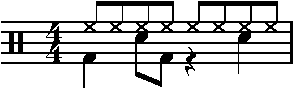
\includegraphics[scale=1.2]{lilypond/example_label.cropped.pdf}};

% Predicted Transcription
\node[
    anchor=west,
    label=north:{\large{Predicted Transcription}}
] (pred) at (0, -0.5cm) {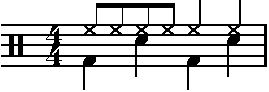
\includegraphics[scale=1.2]{lilypond/example_prediction.cropped.pdf}};


% False Positives
\node[
    anchor=north,
    label={[label distance=0.49cm]north:{\normalsize{\acrfullpl{FP}}}},
] (fp) at (0, -3cm) {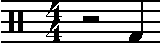
\includegraphics[scale=1.2]{lilypond/example_fp.cropped.pdf}};

% True Positives
\node[
    anchor=north,
    label=north:{\normalsize{\acrfullpl{TP}}},
    left=0.25cm of fp
] {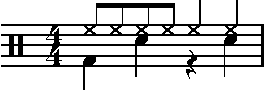
\includegraphics[scale=1.2]{lilypond/example_tp.cropped.pdf}};
    
% False Negatives
\node[
    anchor=north,
    label={[label distance=0.49cm]north:{\normalsize{\acrfullpl{FN}}}},
    right=0.25cm of fp
] {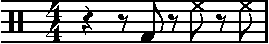
\includegraphics[scale=1.2]{lilypond/example_fn.cropped.pdf}};

\matrix[
    column sep=0.5cm
] at (0, -5cm) {
    \node {\large{\textbf{Classwise F1}:}}; &
    \node[
        label=north:{\large{\acrshort{KD}}}
    ] {\large{0.5}}; &
    \node[
        label=north:{\large{\acrshort{SD}}}
    ] {\large{1.0}}; &
    \node[
        label=north:{\large{\acrshort{HH}}}
    ]{\large{0.86}}; \\
};
\matrix[
    column sep=0.5cm
] at (0, -6cm) {
    \node {\large{\textbf{Macro F1}: 0.79}}; &
    \node {\large{\textbf{Micro F1}: 0.82}}; \\
};


\end{tikzpicture}
    \caption{Illustration of micro and macro F1-score computation for an example \gls{ADT} transcription. Symbols such as \HaPa, \ViPa, and \AcPa denote pauses, and not onsets. Macro F1 reflects the average performance across individual instruments, while micro F1 captures the overall transcription quality across the entire sequence. For clarity, F1-scores are reported with two decimal places.}
    \label{F1Figure}
\end{figure}